\documentclass{tufte-handout}

%\geometry{showframe}% for debugging purposes -- displays the margins

\usepackage{amsmath}

% Set up the images/graphics package
\usepackage{graphicx}
\setkeys{Gin}{width=\linewidth,totalheight=\textheight,keepaspectratio}
\graphicspath{{graphics/}}

\title{Endocrine Control Systems}
\author{Dave Bridges, Ph.D.}
%\date{24 January 2009}  % if the \date{} command is left out, the current date will be used

% The following package makes prettier tables.  We're all about the bling!
\usepackage{booktabs}

% The units package provides nice, non-stacked fractions and better spacing
% for units.
\usepackage{units}

% The fancyvrb package lets us customize the formatting of verbatim
% environments.  We use a slightly smaller font.
\usepackage{fancyvrb}
\fvset{fontsize=\normalsize}

% Small sections of multiple columns
\usepackage{multicol}

% Provides paragraphs of dummy text
\usepackage{lipsum}

% These commands are used to pretty-print LaTeX commands
\newcommand{\doccmd}[1]{\texttt{\textbackslash#1}}% command name -- adds backslash automatically
\newcommand{\docopt}[1]{\ensuremath{\langle}\textrm{\textit{#1}}\ensuremath{\rangle}}% optional command argument
\newcommand{\docarg}[1]{\textrm{\textit{#1}}}% (required) command argument
\newenvironment{docspec}{\begin{quote}\noindent}{\end{quote}}% command specification environment
\newcommand{\docenv}[1]{\textsf{#1}}% environment name
\newcommand{\docpkg}[1]{\texttt{#1}}% package name
\newcommand{\doccls}[1]{\texttt{#1}}% document class name
\newcommand{\docclsopt}[1]{\texttt{#1}}% document class option name

\begin{document}

\maketitle% this prints the handout title, author, and date

\begin{abstract}
\noindent This lecture covers general principles of endocrine control systems.  It covers the following pages in the textbook: 12; 121-124; 319-332\cite{Widmaier2013}.  The goals of this lecture are to demonstrate the basic concepts of endocrinology including what hormones do, how they are classified and generally how they function.  This is the first of seven lectures, the next six of which will go into various endocrine systems in much more detail.  The concepts in this lecture are essential to the understanding of the rest of the lecture.  This series of lectures will focus on the normal physiology and pathophysiology of the endocrine system, but for more information about specific dental-related aspects of endocrine pathophysiology have a look at this paper \cite{Carlos2010}.
\end{abstract}

\tableofcontents

\pagebreak

\section{Learning Objectives}
For this lecture, the learning objectives are:
\begin{itemize}
\item Define endocrine, paracrine, autocrine, and exocrine systems, define neuro-secretory cells by giving a few examples.
\item List major categories of hormones and give several examples that belong to each class.
\item List important factors that determine hormone levels in circulation.
\item Describe four general functions of hormones.
\item Explain with examples neuroendocrine integration.
\item Explain cellular actions of hormones via membrane receptors.
\item Explain cellular action of hormones via transcript and protein synthesis.
\item Discuss major categories of cellular signal pathways of hormones via membrane receptors.
\item Discuss major categories of cellular signal pathways of hormones via cytosolic/nuclear receptors.
\item Define basal secretion and stimulated secretion of endocrine glands.
\item Describe negative and positive feedback system using an example.
\end{itemize}

\section{General Hormonal Principles}
\newthought{A major advantage of multicellularity}, is that biological roles are divided into specialized organs and tissues.  In a single cellular organism, such as \textit{Saccharomyces cerevisiae}\sidenote{also known as brewer's yeast}, all cells need to autonomously be able to sense the environment, cellular conditions and respond appropriately.  Multicellular organisms are able to use more sophisticated mechanisms to sense the environment and make these decisions.  Essential to this division of labor is the ability of these organ systems to communicate efficiently and effectively with each other.  This is accomplished through hormones, which are secreted from one organ to another.

\subsection{Hormonal Classification}

There are hundreds, if not thousands of hormones, if defined loosely to mean \emph{chemicals derived from one cell that can affect another cell}\sidenote{more specifically it can be defined as: "a class of signaling molecules produced by glands in multicellular organisms that are transported by the circulatory system to target distant organs to regulate physiology and behaviour. Hormones have diverse chemical structures that include eicosanoids, steroids, amino acid derivatives, peptides, and proteins -- Wikipedia.}.  Remembering what these all do, how they are made, where they come from can be a challenge.  To simplify this, these can be grouped several ways including chemically, anatomically or functionally.  

\newthought{Chemically,} hormones can be small molecules such as amino acids or lipids, or can be small polypeptides, or even large proteins with three dimensional structures (see Figure \ref{fig:chemical-classification}).  Often, an endocrine organ only releases hormones of a particular chemical class.  An example of this is the adrenal gland which secretes several steroid hormones, each of which have different roles and target tissues.

\begin{marginfigure}
  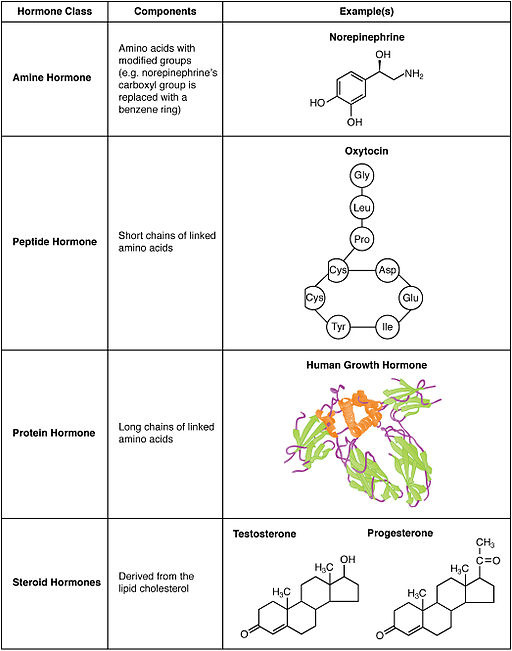
\includegraphics{figures/hormone-classification}
  \caption{Chemical classification of hormones.}
    \label{fig:chemical-classification}
\end{marginfigure}

\newthought{Anatomically,} hormones can be grouped based on where they are secreted from.  Some major exocrine organs include the pancreas, the adrenal gland and the brain.  Another way of considering anatomical classification of hormones is the relationship between the secreting cell and the target cell.  Hormones can act on the secreting cell, or a very close cell or a cell in a (relatively) far away tissue.  These are known as autocrine, paracrine and endocrine actions (see Table \ref{tab:hormone-classification}).

\begin{margintable}
  \centering
  \begin{tabular}{lll}
    \toprule
    Type & Target & Example \\
    \midrule
    Autocrine & Secreting cell & Monocyte IL-1\\
    Paracrine & Nearby cell & Hedgehog \\
    Endocrine & Far away cell & Insulin \\
    \bottomrule
  \end{tabular}
  \caption{Types of hormones, based on the proximity of target and secreting cells}
  \label{tab:hormone-classification}
  %\zsavepos{pos:normaltab}
\end{margintable}

\newthought{Functionally,} one can group hormones together based on collective regulation  of a set of organs.  These are often considered \emph{axes} and some examples include the hypothalamic-pituitary-adrenal (HPA) axis, gut-liver-brain axis or the sympathetic -adrenal-medullary (SAM) axis. 

\section{Hormonal Signaling Concepts}

All hormones can be understood best from a general framework of understanding swhat regulates the levels of the hormone in the body, and how and where it exerts its actions.  For each hormone we will examine in this unit, we will discuss the following points

\begin{itemize}
\item Where is the hormone made?
\item What signals cause that hormone to be released?
\item What are the receptors and signaling cascades activated by this hormone?
\item What tissues does this hormone affect, and how?
\item How is the signal turned off
\end{itemize}

\subsection{Regulation of Hormone Levels}

Most signaling events are controlled at the level of hormonal secretion.  When the pancreas wants to communicate with the liver, it can secrete insulin or glucagon from storage vesicles.  This can occur very rapidly, as long as sufficient hormone is present in the storage vesicles and the liver receptors are sufficiently prepared to respond.

\newthought{Synthesis and processing of hormones} generally occurs from a specific cell type in a particular gland.  Normally endocrine glands\sidenote{as opposed to an exocrine gland, which releases its contents externally.  These would include salivary, mammary and sweat glands} allow for release of stored hormones into the blood in response to a particular signal.  Typically these glands synthesize the hormone, process it into an active form and store it in a state where it can be released on demand.  The major glands that release hormones are the pineal, pituitary, thyroid and parathyroid glands, as well as the pancreas, ovaries, testes, hypothalamus and adrenal glands.  Peptide and protein hormones can be regulated at the transcriptional level, translational level or via regulation of post-translational processing or directed vesicular secretion.  Steroid hormones are often controlled by enzymatic activation of their synthetic pathways and released in response to specific exocytotic signals.  

\begin{marginfigure}
  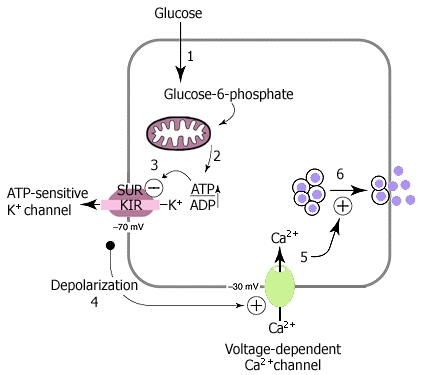
\includegraphics{figures/insulin-secretion}
  \caption{Mechanisms of glucose-induced insulin secretion from pancreatic $\beta$-cells.}
    \label{fig:insulin-secretion}
\end{marginfigure}

\newthought{Some hormones are secreted upon stimulation, wheras others are released basally and without stimulus.}  In the case of basal secretion, the hormone is released at all times, as soon as it is made and processed.  Some examples of constitutive secretion are growth hormone\sidenote{As we will discuss in lecture 4, GH is actually a mixture of basal secretion along with secretion regulated by GHRH (Growth Hormone Releasing Hormone) and somatostatin} and prolactin release.  In these cases this maintains a steady level of hormone release, often to maintain long-term processes such as growth.  As is the case with both GHRH and prolactin, basal secretion can also be augmented if necessary by other signals.

\newthought{Regulated secretion of hormones} occurs in response to an initiating signal.  In these cases the hormone is synthesized and stored in prepration for a secretion signal.  For example, in the case of insulin the pancreatic $\beta$-cells sense increases in blood glucose levels, causing a depolarization of the plasma membrane via ATP-sensitive potassium channels and allowing for exocytosis of insulin storage granules.  This is described in Figure \ref{fig:insulin-secretion}.  This can continue as long as there is enough insulin storage granules.  Most hormones have specific signaling/sensing pathways that regulate their synthesis and secretion.  Some examples of these are shown in Table \ref{tab:secreting-events}.

\begin{margintable}[-1cm]
  \centering
  \begin{tabular}{ll}
    \toprule
    Signal & Examples \\
    \midrule
    Neural Stimuation & Adrenalin, CRH, TSH \\
    Another Hormone & Cortisol, Thyroid Hormones \\
    Metabolite & Insulin, Glucagon, Calcitonin \\
    Physical Stimuli & Ghrelin, Renin \\
    \bottomrule
  \end{tabular}
  \caption{Some examples of mechanisms by which hormone release can be stimulated.}
  \label{tab:secreting-events}
  %\zsavepos{pos:normaltab}
\end{margintable}

\subsection{Principles of Hormone Receptors}

\newthought{All hormones have receptors}, either on the surface of the cell (if the hormone is not membrane soluble) or on the inside of the cell (if the hormone can cross the plasma membrane).  Receptors have two key features, they must \emph{recognize} the hormone and they must be able to \emph{transmit} that recognition event.

\newthought{Hormones are recognized} by specific receptors, and can be thought of as key/lock pairs.  For example the feeding hormone Leptin binds to the Leptin Receptor in the hypothalamus, causing suppression of appetite.  If either of these genes are mutated then the subject is hyperphagic.  Some hormones can bind to several receptors, and some receptors are capable of binding one or more hormones, increasing the potential complexity of the signaling system.  When trying to understand a hormonal signaling event, it is useful to think of what the receptors are, and where they are located.  

Generally hormone receptors can be grouped into cell-surface receptors and nuclear hormone receptors.  Cell surface receptors detect the hormone signal at the cell surface then propagate that signal by activating second messengers and protein phosphorylation cascades to modify the activity of target proteins.  Nuclear hormone receptors bind to the hormone \emph{after it enters the cell}.  Typically these hormones activate the receptor allowing for it to translocate to the nucleus and bind specific DNA targets (see Figure \ref{fig:nuclear-hormone-receptors}, modified from \cite{Chen1999}).  These hormones typically regulate the transcription of target genes and therefore are slower acting than cell surface receptors.

\begin{marginfigure}[-14cm]
  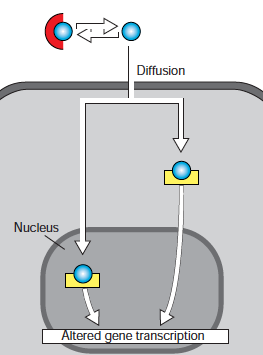
\includegraphics{figures/nuclear-hormone-receptors}
  \caption{Mechanisms of nuclear hormone-receptor signal transduction.}
    \label{fig:nuclear-hormone-receptors}
\end{marginfigure}

\newthought{The tissue distribution of hormone receptors} is key to understanding what physiological effects the hormone may exert.  As an example, insulin receptors cause dramatically different physiological effects depending on the target tissue (see Table \ref{tab:insulin-tissue-roles}).

\begin{table}
  \centering
  \begin{tabular}{ll}
    \toprule
    Tissue & Effect \\
    \midrule
    Pancreas & Blocks insulin secretion \\
    Liver & Prevents gluconeogenesis, promotes glycogenesis\\
    Fat & Glucose uptake, lipid synthesis \\
    Hypothalamus & Reduces appetite \\
    \bottomrule
  \end{tabular}
  \caption{Some examples of tissue-specific effects of insulin in various tissues.}
  \label{tab:insulin-tissue-roles}
  %\zsavepos{pos:normaltab}
\end{table}

Understanding what a hormone does, therefore is highly dependent on the tissue what it is acting on.  Several of the hormones we will discuss in the next few lectures function through G$_{s}$-linked G-Protein Coupled Receptors which work by synthesizing cAMP and activating the protein kinase PKA.  In each of these cases, PKA gets activated, but the results of PKA activation differ from cell to cell.

\newthought{Hormones can regulate} a wide variety of cellular processes.  Two of these include changing metabolism rapidly via post-translational modification of key enzymes, and directing the synthesis of new transcripts, resulting in longer lasting changes in cellular physiology.  For example, if a cell needs to rapidly respond to a stress signal such as adrenaline, a fast-acting second-messenger pathway\sidenote{In this case it is a G-Protein Coupled Receptor mediated activation of cAMP-dependent signaling} is activated to quickly accelerate muscle contraction.  If long term changes to  are required, such as the case in sex hormones, testosterone can alter transcriptional pathway.\sidenote{testosterone  binds to the androgen receptor, a nuclear hormone receptor.}
% come up with some examples of short term and long term changes


\subsection{Negative and Positive Feedback of Hormones}

Although we think quite a lot about how a hormone signaling event is initiated, just as important is the processes by which we end the event.  For example, adrenaline will acellerate our heart rate but if that went on indefinitely we would develop arrhythmia.  There are two main ways in which endocrine processes can be stopped;  you can reduce the amount of the circulating hormone, or you can alter the responsiveness of the target tissue.  In most cases both of these processes occur.

\newthought{Negative feedback of signal transduction events} is the primary mechanism by which a target cell can stop responding to a hormone.  In the case of G-Protein coupled receptors, there is a class of compounds called arrestins that mediate this process (see Figure \ref{fig:arrestins}, modified from \cite{Lefkowitz2005}).  In this paradigm, after GPCR activation a class of kinases called GRKs (G-Protein Coupled Receptor Kinases) phosphorylate the receptor, which recruits the arrestins.  The arrestin molecules now sterically prevent further G-protein activation, and further signaling from that receptor.  In other cases, the cell surface receptors may be internalized or degraded or the ability of signals to be propagated from those receptors may be blocked.

\begin{marginfigure}[-13cm]
  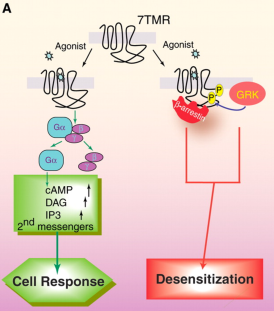
\includegraphics{figures/arrestins}
  \caption{Arrestin mediated negative feedback of GPCR signaling.}
    \label{fig:arrestins}
\end{marginfigure}

\newthought{Reduction of serum hormone levels can occur by stopping production or release of new hormones or by degrading or removing the existing hormone.}  In the case of cortisol signaling, its release is caused by the sequential upstream release of CRH and ACTH.  Along with its effects on its intended target tissues, cortisol also acts on the pituitary and the hypothalamus to prevent the synthesis of ACTH and CRH respectively.  

Separate to this feedback mechanism, in many target tissues, cortisol also induces the synthesis of an enzyme called 11$\beta$-hydroxysteroid dehydrogenase type 2.  This enzyme converts cortisol to its less active metabolite cortisone \cite{Hubener1956}.  This effectively reduces the cortisol levels within the target cell.  In this way cortisol both reduces its synthesis (through repression of ACTH/CRH) and induces its own breakdown (through 11$\beta$-hydroxysteroid dehydrogenase type 2).

\newthought{Most endocrine loops have built-in negative feedback circuits.}  If they did not then hormonal signaling would occur in an unrestrained manner.  On the other hand, too much negative feedback can also be a bad thing.  In the case of insulin signaling, too much insulin action (for example as in the case of over-eating) can lead to chronic insulin resistance.  This in turn leads to an inability of the body to correctly dispose of glucose efficiently, eventually resulting in type II diabetes.  We will discuss this in more detail in the lecture on pancreatic function and metabolic control.

\newthought{Another type of feedback is positive feedback.}  This is less common, and results in a hormone that responds to a stress and then functions in a way to amplify its own release.  An example of this is oxytocin which is released during delivery.  This hormone is released by the mother's pituitary and the fetus and causes contractions of the uterine lining.  This stretch is sensed by the pituitary, causing more oxytocin to be released.  This circuit will result in increasing amounts of both contractions and oxytocin.  As with most positive feedback loops, this effect is inherently unstable and requires an external event (in this case, the delivery of the fetus) for the loop to stop self-promoting.

\section{Neuroendocrinology}

Many hormonal signaling events involve the brain, which could be considered the most complex and central endocrine organ.  The primary role of the brain is to integrate external sensory cues with internal signals and to decide, often subconsciously the most appropriate response.  The key parts of the brain that are involved in endocrine responses are the hypothalamus and the pituitary (Figure \ref{fig:pituitary-hypothalamus}).

\begin{marginfigure}
  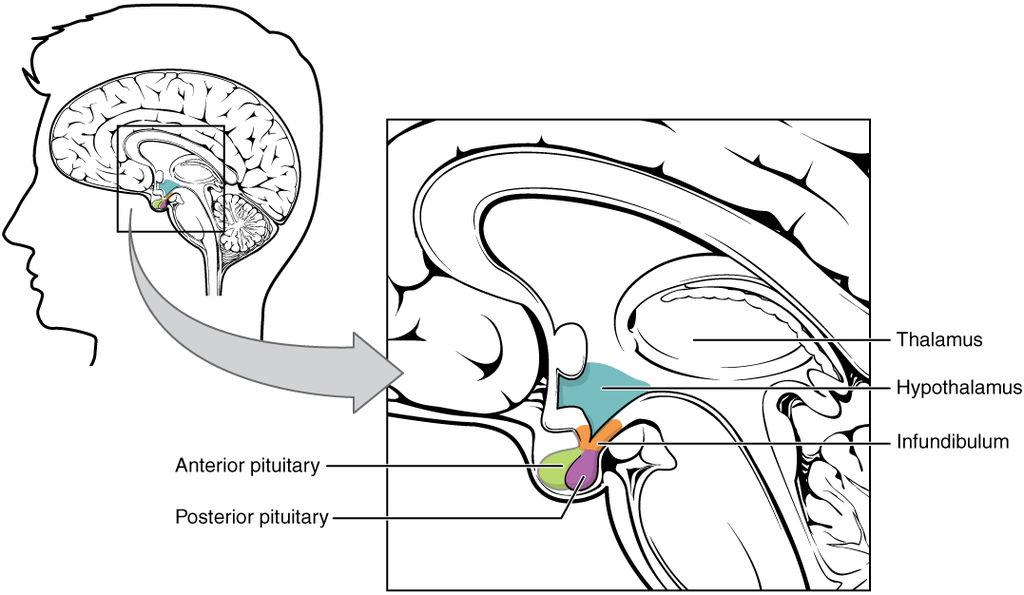
\includegraphics{figures/pituitary-hypothalamus}
  \caption{Location of the pituitary and hypothalamus in the human brain.}
    \label{fig:pituitary-hypothalamus}
\end{marginfigure}

\newthought{The Hypothalamus\sidenote{Under the thalamus}} often responds to hormones sent from either the periphery or the rest of the brain.  This makes it the link between the nervous and the endocrine systems.  The hypothalamus is a central node for the regulation of appetite, circadian rhythyms, body temperature and behaviors.  The hypothalamus can signal to other parts of the brain, including the pituitary gland making it the crossover point of the endocrine and nervous systems.  We will discuss the role of the hypothalamus more in the second and third lectures.  Several endocrine circuits exploit the proximity of these two brain regions (see Table \ref{tab:pituitary-axes}):

\begin{table}
  \centering
  \begin{tabular}{lccl}
    \toprule
    Axis & Hypothalamic & Pituitary & Function \\
    \midrule
    HPA & CRH & ACTH & Glucocorticoids \\
    HPG & GnRH & FSH/LH & Reproductive hormones \\
    HPT & TRH & TSH & Thyroid hormones \\
    \bottomrule
  \end{tabular}
  \caption{Pituitary-hypothalamic axes.}
  \label{tab:pituitary-axes}
  %\zsavepos{pos:normaltab}
\end{table}

\newthought{It is important the nervous system is able to integrate with the endocrine system.}  Some endocrine responses, such as adrenaline and cortisol secretion are activated by nervous activity.  Other hormones such as ghrelin and leptin, which modify appetite, start as signals in the periphery but then function on the nervous system to alter behaviors.  When considering \textit{a priori} whether a hormone has a neuroendocrine role, take into account whether this hormone is either the cause of, or is in response to a process regulated by the brain.  If that is the case, then it is likely that the hypothalamus has receptors for this hormone and plays a role in co-ordinating those effects.

\listoffigures
\listoftables

\bibliography{library}
\bibliographystyle{plainnat}



\end{document}
